\section{Calibration}
Put short description.

%%%%%%%%%%%%%%%%%%%%%%%%%%%%%%%%%%%%%%%%%%%%%%%%%%
\subsection{Channel-by-Channel Calibration}
%%%%%%%%%%%%%%%%%%%%%%%%%%%%%%%%%%%%%%%%%%%%%%%%%%

800 MeV/$c$ $\pi~+$ is expected to pass-through the 76 cm
of TPC fiducial volume with almost uniform energy deposition.
So it cau be used to calibrate relatvce response of the TPC
signal charge channel-by-channel. 
Figure~\ref{fig:PionTrack} shows trajectry of the 800 MeV/$c$ $\pi^+$
reconstructed by the hit finding and clustering algorithm (See Section \ref{xxx}).
This figure is obtained from $\sim$300 events of well-selected Pion passing-through the TPC.
Pion is triggered by the 5 cm$\times$5 cm BDC located in front of the 250L vessel (See Figure~\ref{K11Br_Beam_line}), 
beam size is consistent with 5 cm ($\sim$ 65 $\mu$s in drift time) at the injection point.
Then it gradually spread while pion travels through the TPC because of the multiple scattering.

Figure~\ref{fig:PionQvsCh} shows the hit charge as a function of the TPC channel number
obtained from the same $\pi^+$ data. Grayscale contours show hit charge distributions for
each channel and black points correspond to average of the hit charge distribution.  
Aothough we expect the energy deposition of the through-going pion to be uniform,
we observe relatively large channel dependence. 
Detailed study of the non-uniformity will be discussed in section xx, in summary,  
this is mainly because of the distortion of the TPC drift field.
We use this average charge as channel-by-channel normalization scale.
The response becames flat in Fig.~\ref{fig:PionQcvsCh} after applying the normalization.
We apply the same normalization procedure for Kaon, Proton, and Cosmic data analysis.


\begin{figure}[htbp]
 \begin{center}
  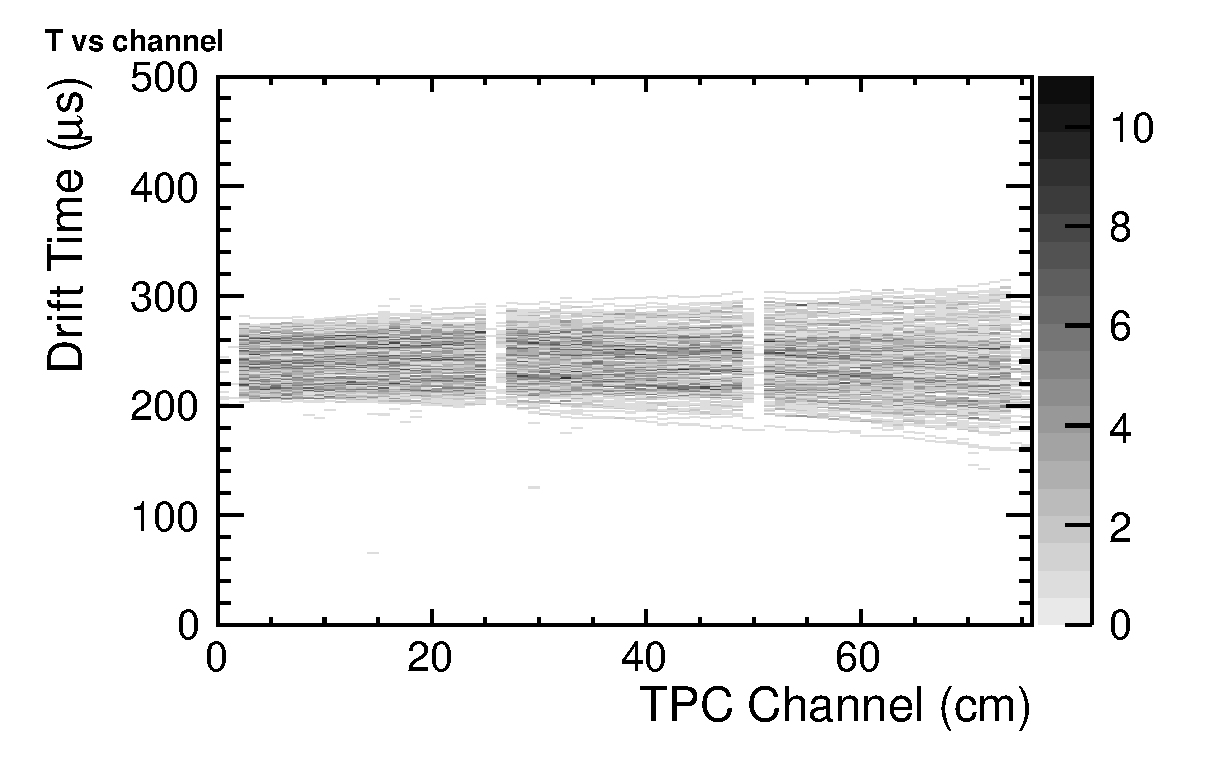
\includegraphics[width=100mm]{fig/PionTrack.eps}
 \end{center}
 \caption{800 MeV/c pion sample}
 \label{fig:PionTrack}
\end{figure}

\begin{figure}[htbp]
 \begin{center}
  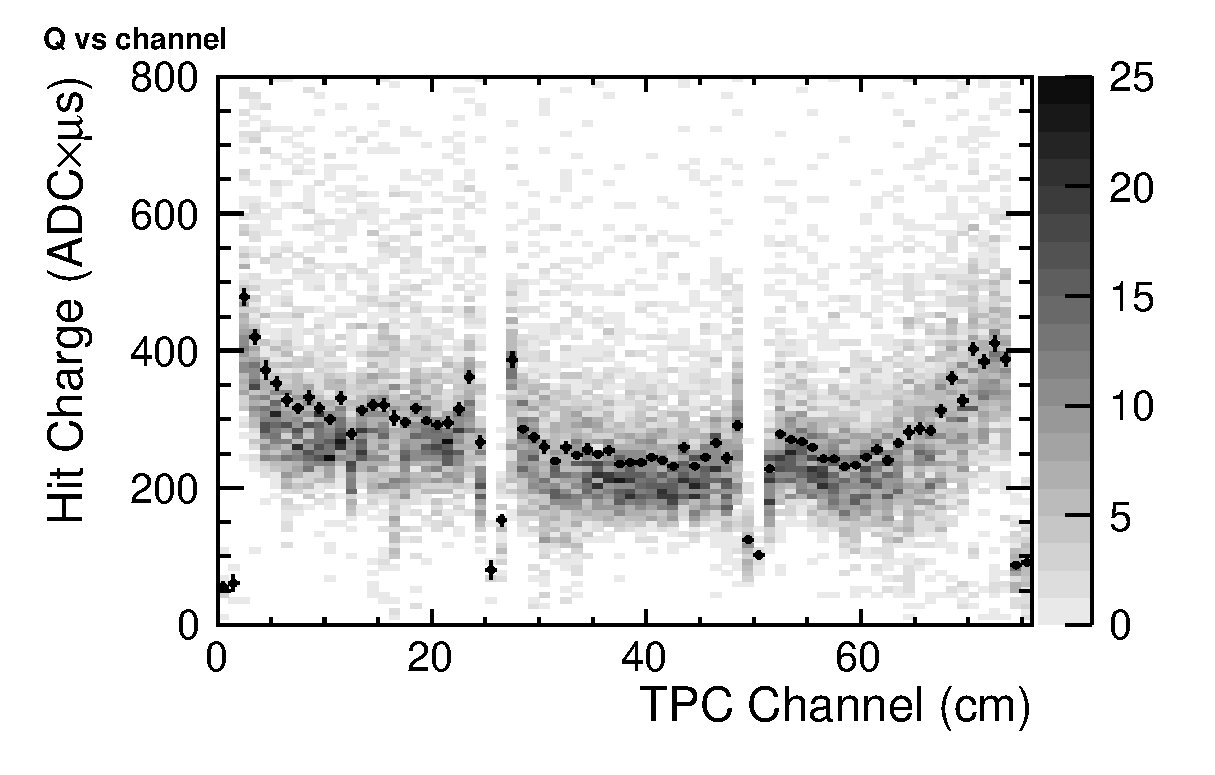
\includegraphics[width=100mm]{fig/PionQvsCh.eps}
 \end{center}
 \caption{800 MeV/c pion average hit charge}
 \label{fig:PionQvsCh}
\end{figure}

\begin{figure}[htbp]
 \begin{center}
  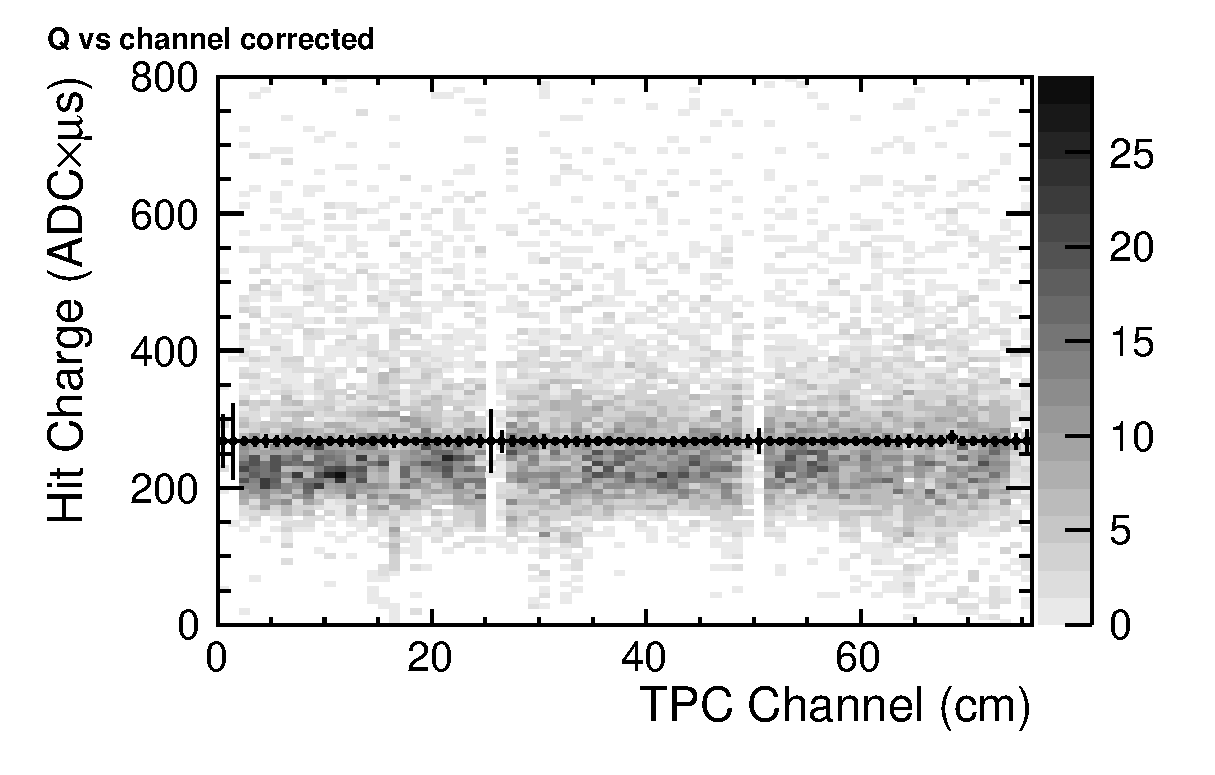
\includegraphics[width=100mm]{fig/PionQcvsCh.eps}
 \end{center}
 \caption{800 MeV/c pion average hit charge after calibration}
 \label{fig:PionQcvsCh}
\end{figure}


%%%%%%%%%%%%%%%%%%%%%%%%%%%%%%%%%%%%%%%%%%%%%%%%%%
\subsection{Liquid Argon Purity}
%%%%%%%%%%%%%%%%%%%%%%%%%%%%%%%%%%%%%%%%%%%%%%%%%%

Attenuation of the drift electron depends on purity of LAr since electronegative impurities capture it \cite{purity}. 
Thus we need to apply correction to TPC signal charge according to the drift time.
We use cosmic ray events triggered by inner PMT at off-beam timing for measuring the LAr purity, and use this to correct the beam data.
Figure~\ref{fig:CosmicEvent} shows an event display of typical cosmic muon event crossing TPC channels.
The attenuation of readout charge depending on drift time is clearly seen in the right plot. 
%Readout charge in an event cannot be fitted by exponential because energy deposition follows Landau distribution and charge readout is affected by electric field distortion which is described latter in section~\ref{sec:Efield}.
Other effects on readout charge are Landau nature in energy deposition and electric field distortion as discussed in the previous subsection.
We use multiple events to cancel Landau effect and apply channel response correction to estimate LAr purity.

%\begin{itemize}
%\item Plot: Typical Lifetime Fit  (Naganoma)
%\item Plot: Lifetime vs Time  (Naganoma)
%\end{itemize}

\begin{figure}[htbp]
 \begin{center}
  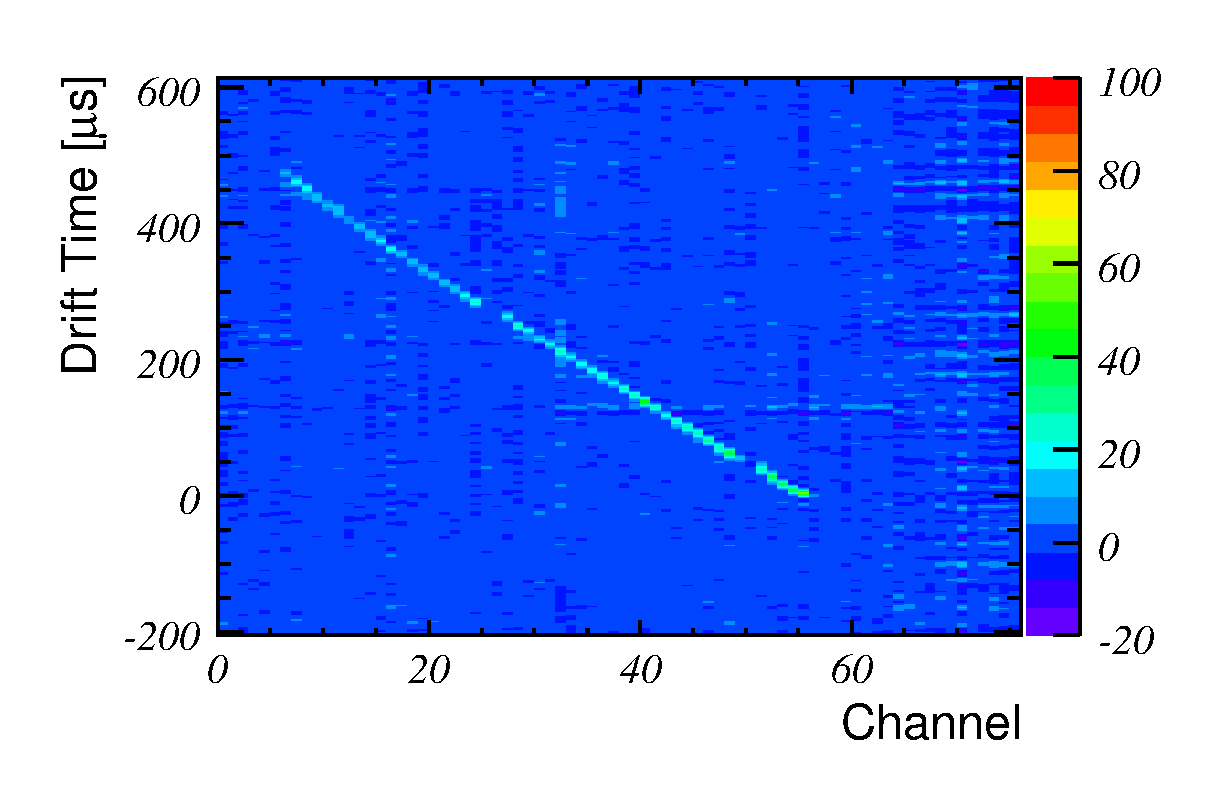
\includegraphics[width=60mm]{fig/cosmic68_ev258_display.eps}
  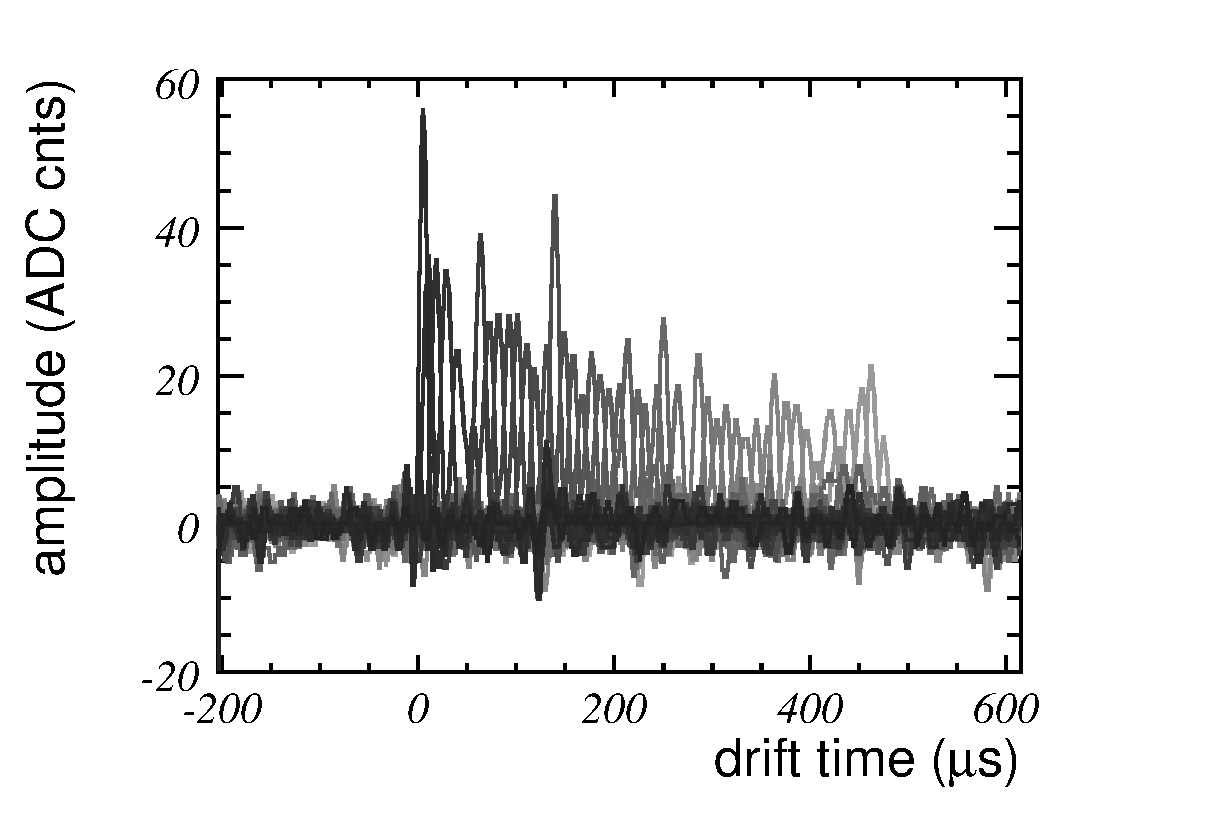
\includegraphics[width=60mm]{fig/cosmic68_ev258.eps}
 \end{center}
 \caption{Left: Typical cosmic muon event crossing TPC channels. Right: Charge deposit as a function of drift time.}
 \label{fig:CosmicEvent}
\end{figure}

We select cosmic ray event with more than 20 TPC channels which corresponds to zenith angle of more than $27^\circ$ and consistent with straight line by $\chi^2$ fit. 
Readout charge is corrected for field distortion and projected to beam direction to correct injection angle.
We fit readout charge by Landau function in each drift time bin to estimate average charge deposit. 
Figure~\ref{fig:tauExample} shows example of the average readout charge as a function of drift time which is fitted by exponential to obtain drift electron lifetime. 
%Realistic Monte Carlo simulation shows about 13\% (TBU) smaller lifetime estimation due to noise, field distortion, and FFT effects. 
%We correct output lifetime from these effects.
Figure~\ref{fig:CosmicPurity} shows an drift electron lifetime as a function of duration after initial LAr filling.
Drift electron lifetime was 600 $\mu$s at 60 hours, and 400 $\mu$s after 150 hours.
%Initial purity looks good, but the purity was slowly degrading while data taking period.
The degradation is possibly due to impurity from micro leak or out-gassing penetrating faster than purification by gas recirculation.
But we kept enough drift electron lifetime during data taking period.
The effects from noise, field distortion, and FFT give about 10\% (to be confirmed) of systematic uncertainty in LAr purity estimation.
Since charge in simulation is calibrated using through-going $\pi$ data as described later and duration of analyzed beam data is short (about 30 hours), this uncertainty gives negligible effects (to be updated, show percentage) in beam data analysis. 

\begin{figure}[htbp]
 \begin{center}
  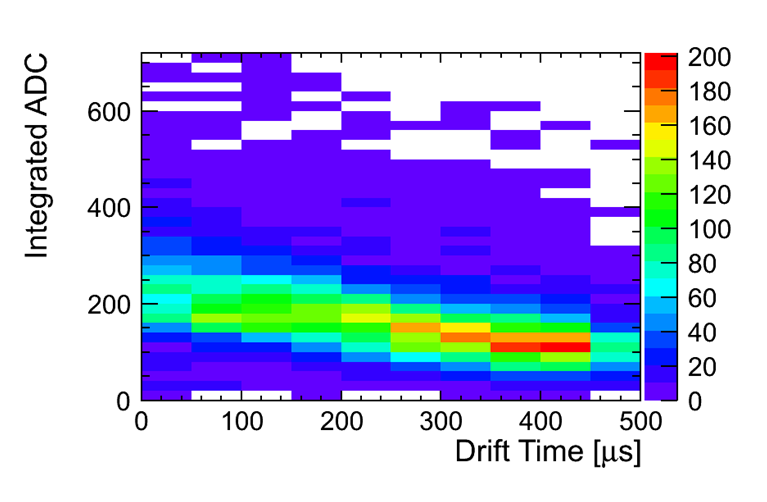
\includegraphics[width=60mm]{fig/chargeDep.eps}
  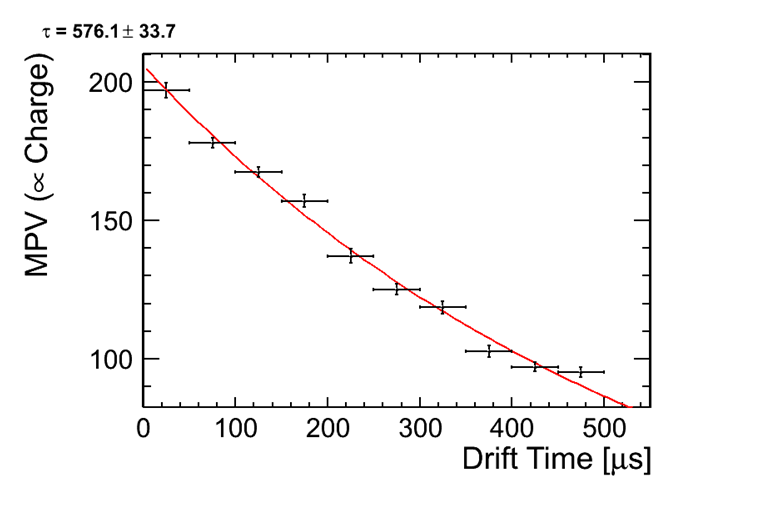
\includegraphics[width=60mm]{fig/tauExample.eps}
 \end{center}
 \caption{Left: Readout charge as a function of drift time. Readout charge in each drift time bin is fitted by landau function. Right: Average charge readout as a function of drift time which is fitted by exponential to estimate drift electron lifetime.}
 \label{fig:tauExample}
\end{figure}


\begin{figure}[htbp]
 \begin{center}
  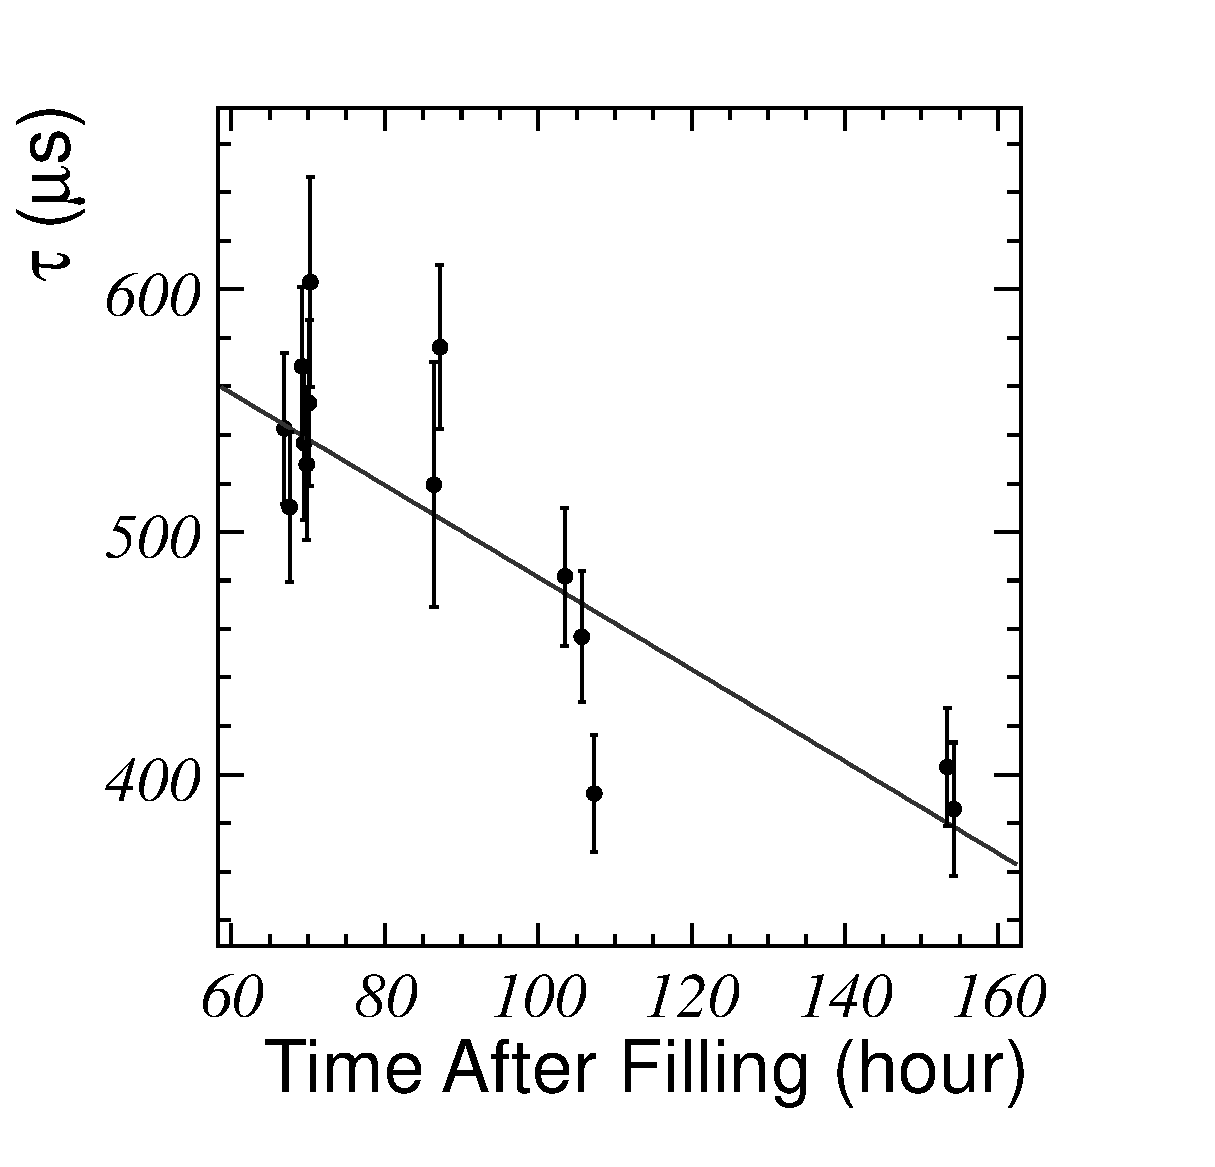
\includegraphics[width=50mm]{fig/tauHistory.eps}
 \end{center}
 \caption{Drift electron lifetime as a function of duration after initial LAr filling. The lifetime is used to correct the beam data.}
 \label{fig:CosmicPurity}
\end{figure}

